\section{Complexity of Nonlinear Fourier Transform}

% \subsection{\acrlong{nft}}

Computational complexity is one of the most important parameters of processing systems. Number of \acrfull{flop} is used to evaluate this parameter. To assess complexity in telecommunications, the \acrshort{flop}s per symbol or per bit of transmitted information is used. Fig.~\ref{fig:complexity}a shows the value of \acrshort{flop}s per symbol for the \acrshort{fnft} method depending on the number of samples per symbol (SpS). As expected, the complexity increases with the number of symbols transmitted, as the overall signal length grows. As SpS increases, the graph shifts upward, since the number of points in the signal increases proportionally. Fig.~\ref{fig:complexity}b shows a comparison of the complexity of \acrshort{fnft} and \acrshort{dbp}. This graph shows the value of \acrshort{flop}s per bit. The graph shows the \acrshort{fnft} method without additional estimation of the complexity for the PJT method and the complexity of calculating the normalization factors for the discrete spectrum.
%We expect the complexity of the methods to contribute little to the overall complexity.
The graph shows that the complexity of the \acrshort{nft} is several times greater than the complexity of the \acrshort{dbp}. However, the complexity of the \acrshort{nft} is independent of the fiber length.

The peculiarity of estimating the number of operations for searching for discrete eigenvalues is that it depends on the signal power. At higher power, there are more points in the continuous spectrum, therefore the algorithm works longer. For PJT, the number of operations can be estimated as follows: we can multiply the number of discrete eigenvalues by the average of the number of operations to calculate one eigenvalue. The minimum number of operations can be achieved using the Ablowitz-Ladik method, which gives us $49 N$ operations to calculate one coefficient $a(\xi)$.
% From our research, we can estimate that the average number of calculations of the coefficient is in the range from 10 to 100 and depends on the signal power.

For example, our research shows that for 2048 symbols, with an average power of 0 dBm, about $10^5$ additional calculations of the coefficients $a(\xi)$ are required. The number of discrete eigenvalues is about $10^3$. As a result, $10^5 \cdot 49 N$ operations will be added to the \acrshort{flop}s for calculating the continuous spectrum. Then the number of operations for the bi-directional algorithm for calculating the phase coefficients is added to this number. It is equal to the number of eigenvalues multiplied by the number of operations to calculate one coefficient: $10^3 \cdot 152 N$ \acrshort{flop}s. With 2048 symbols and SpS = 2, the number of points in the signal is $N = 2 \cdot 2^{11}$, which means in addition to the \acrshort{flop}s per symbol shown in Fig.~\ref{fig:complexity}, $10^5 \cdot 50.5 \cdot 2 \approx 10^7$ operations are added. This shows that the main computational costs are spent on calculating the discrete spectrum and phase coefficients. As a solution to this problem, adaptive and fast algorithms can be used to reduce the number of operations. For this it is necessary to develop a fast bi-directional algorithm scheme.

We assume the number of operations for the inverse problem to be equal to the number of operations for the direct problem, up to a coefficient. The main costs are required for the Darboux method, the number of operations for which is proportional to $N^2$.


\begin{figure}[htbp]
\begin{minipage}[h]{.49\linewidth}
    \center{
        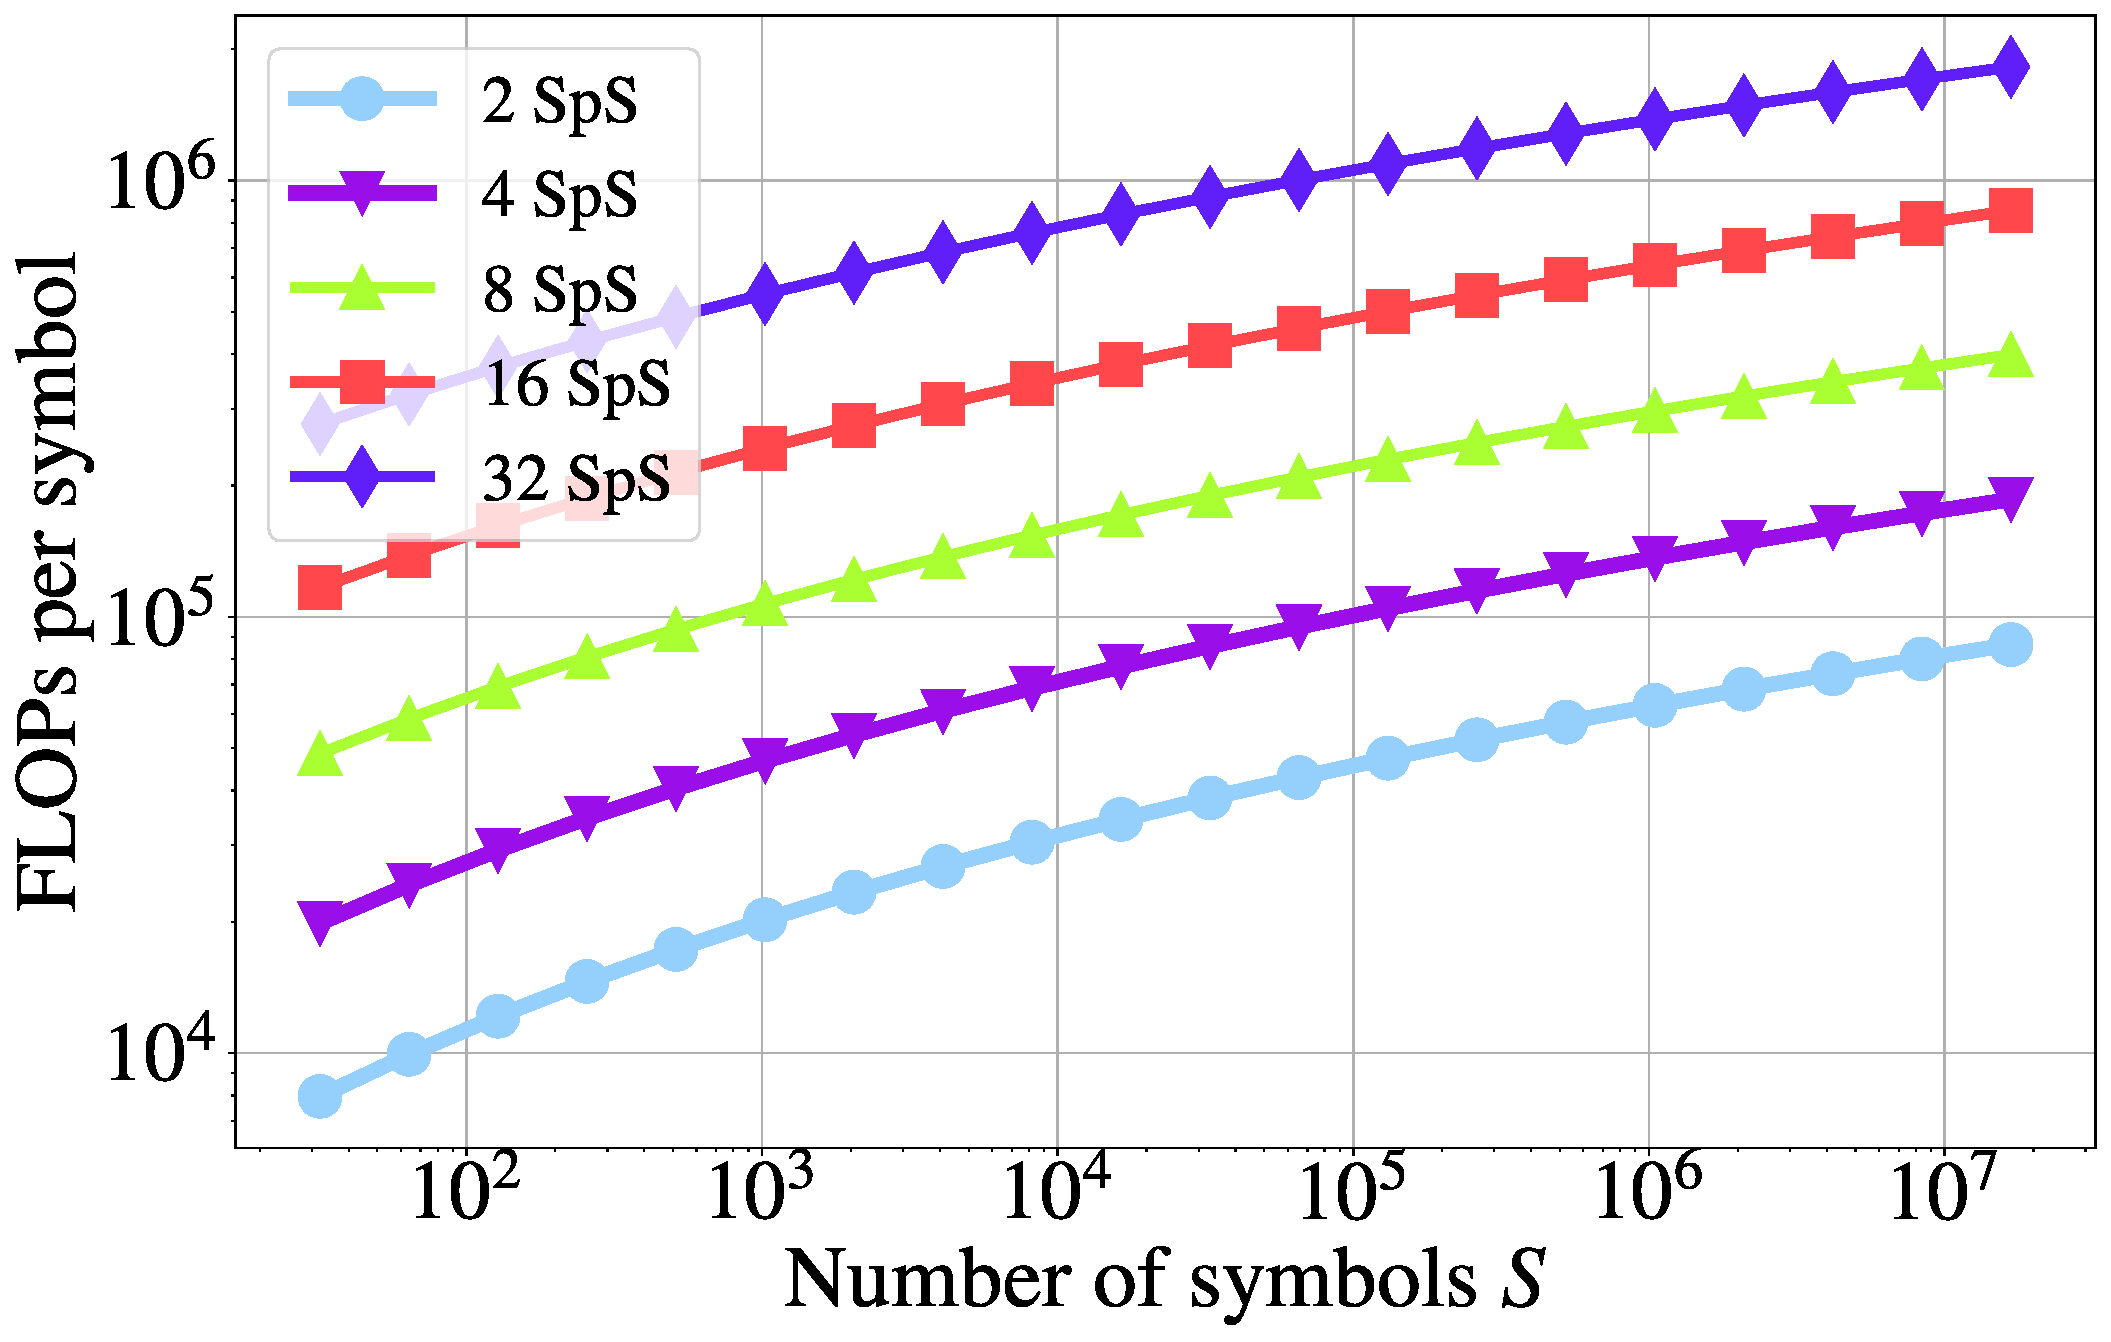
\includegraphics[width=1\linewidth]{images/complexity/complexity_per_symbol.pdf} \\ \textbf{(a)}
    }
	% \label{fig:complexity_per_symbol}
\end{minipage}
\begin{minipage}[h]{.49\linewidth}
    \center{
        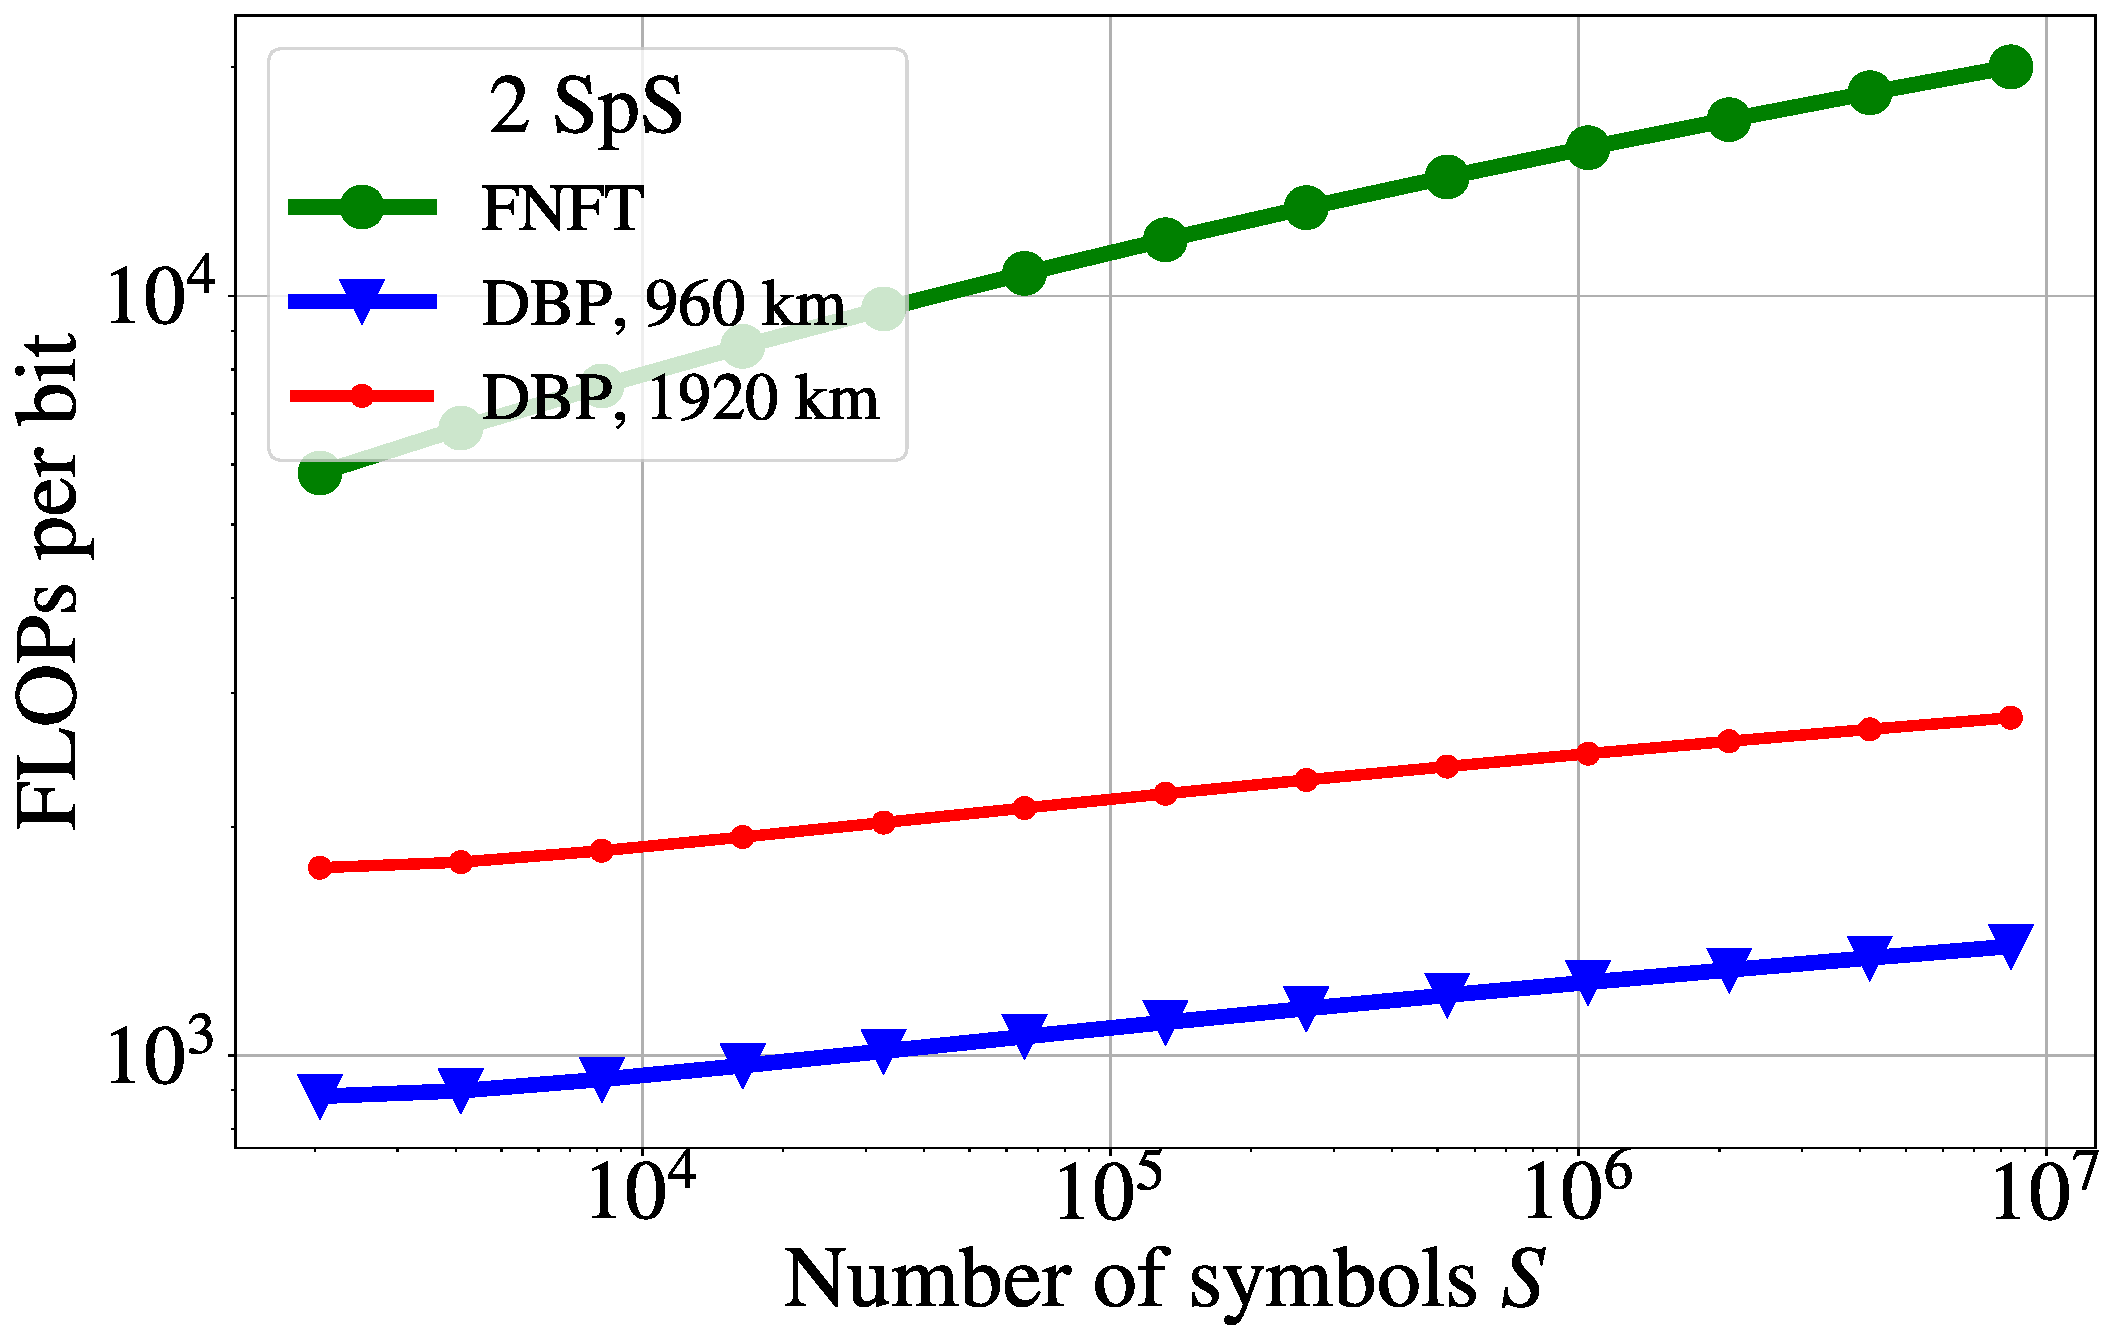
\includegraphics[width=1\linewidth]{images/complexity/complexity.pdf} \\ \textbf{(b)}
    }
	% \label{fig:complexity_dbp}
\end{minipage}
	\caption{Complexity comparison. \textbf{(a)} Number of \acrshort{flop}s per transmitted symbol for different number of samples per symbol (SpS) for the \acrshort{fnft} method. \textbf{(b)} Number of \acrshort{flop}s per transmitted bit for \acrshort{dbp} and \acrshort{fnft} methods (SpS = 2).}
	\label{fig:complexity}
\end{figure}


% \subsection*{PJT Complexity}

% Here is an analysis of the operating time of the discrete spectrum search method -- PJT. The number of calls to integrators of the Zakharov-Shabat problem for tracking grows with an increase in the size of the discrete spectrum. For large values of average power, this stage turns out to be the longest.
% The number of integrator calls for tracking in the current implementation of the PJT grows in proportion to the energy of the discrete spectrum. With its increase, the length of the tracks to discrete eigenvalues grows.

% \begin{figure}[h]
% 	\centering
% 	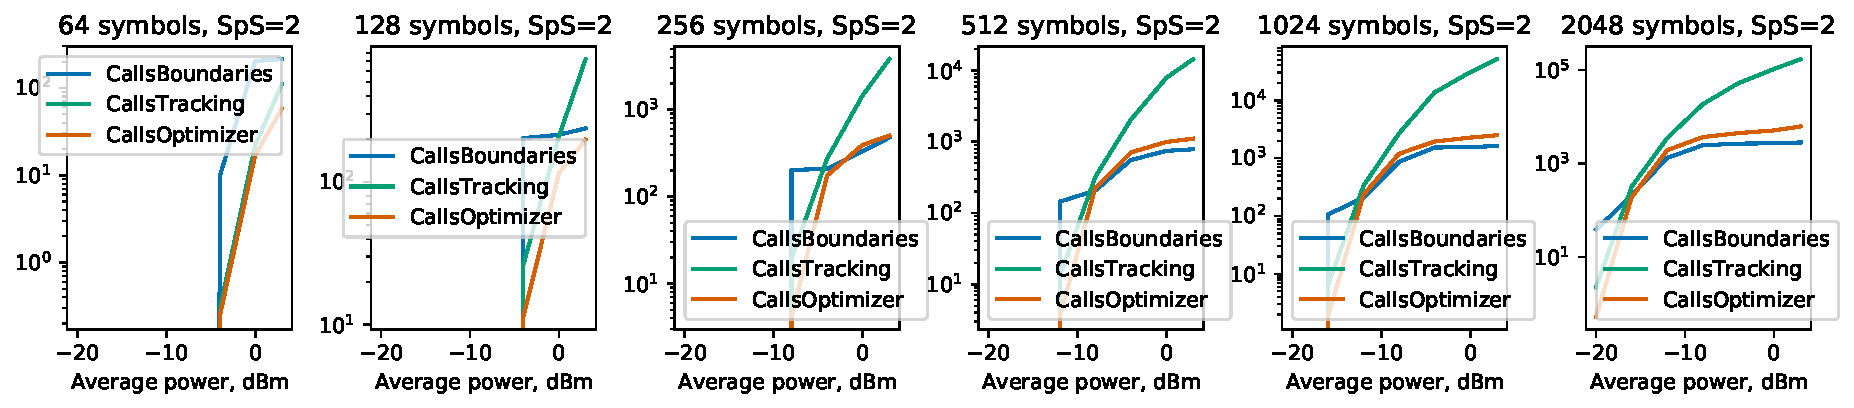
\includegraphics[width=1\linewidth]{images/complexity/PJT_calls_132.pdf}
% 	\caption{PJT: number of integrator calls for different steps: 1) boundaries (except the real axis), 2) tracking along phase jumps, 3) refinement by Muller's method.}
% 	\label{fig:PJTTelecom1}
% \end{figure}

% \begin{figure}[h]
% 	\centering
% 	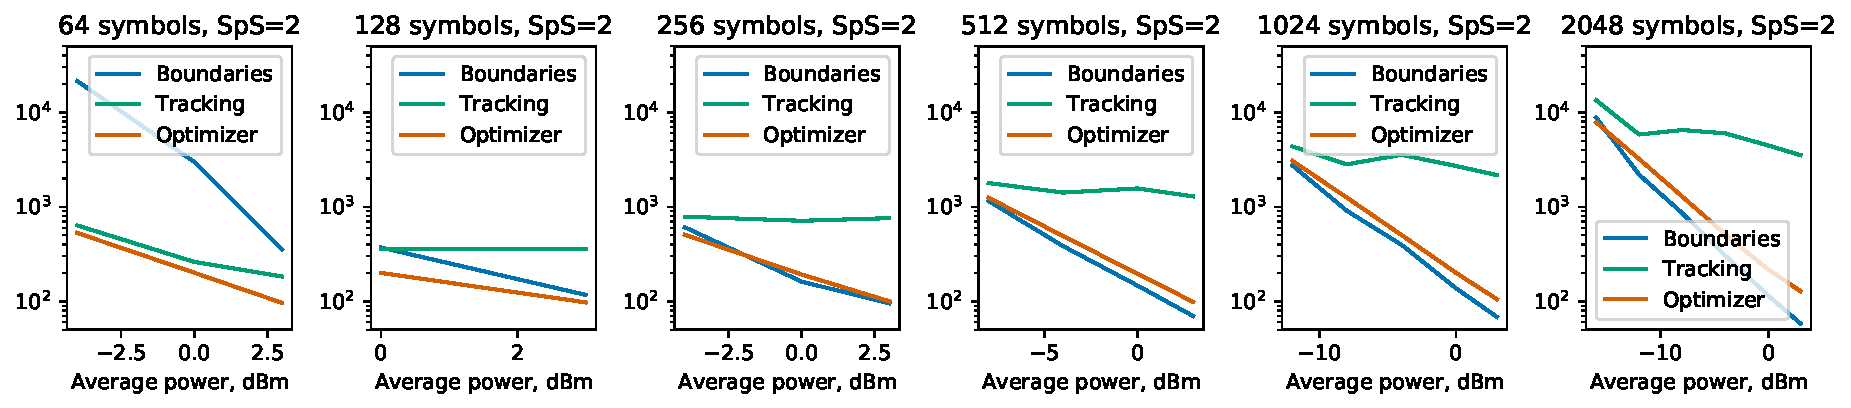
\includegraphics[width=1\linewidth]{images/complexity/PJT_callsPerDirectEnD_132.pdf}
% 	\caption{PJT: number of integrator calls for different steps normalized by discrete spectrum energy $E_D$.}
% 	\label{fig:PJTTelecom2}
% \end{figure}

% \begin{figure}[h]
% 	\centering
% 	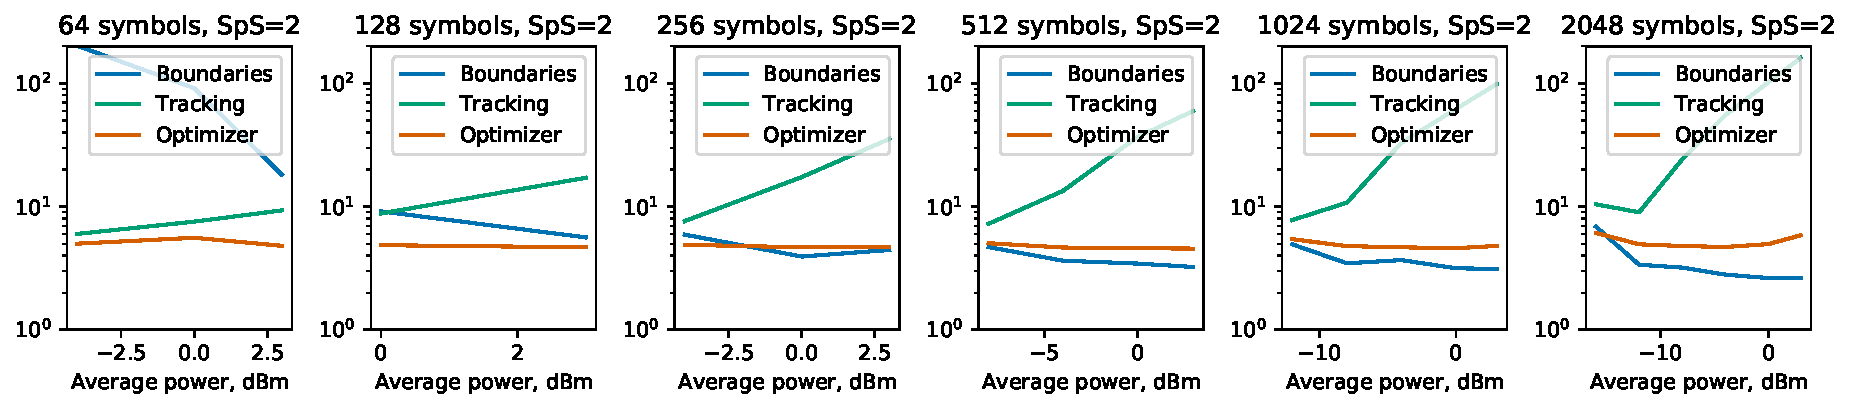
\includegraphics[width=1\linewidth]{images/complexity/PJT_callsPerDSSize_132.pdf}
% 	\caption{PJT: number of integrator calls for different steps normalized by discrete spectrum size.}
% 	\label{fig:PJTTelecom3}
% \end{figure}

% \begin{figure}[h]
% 	\centering
% 	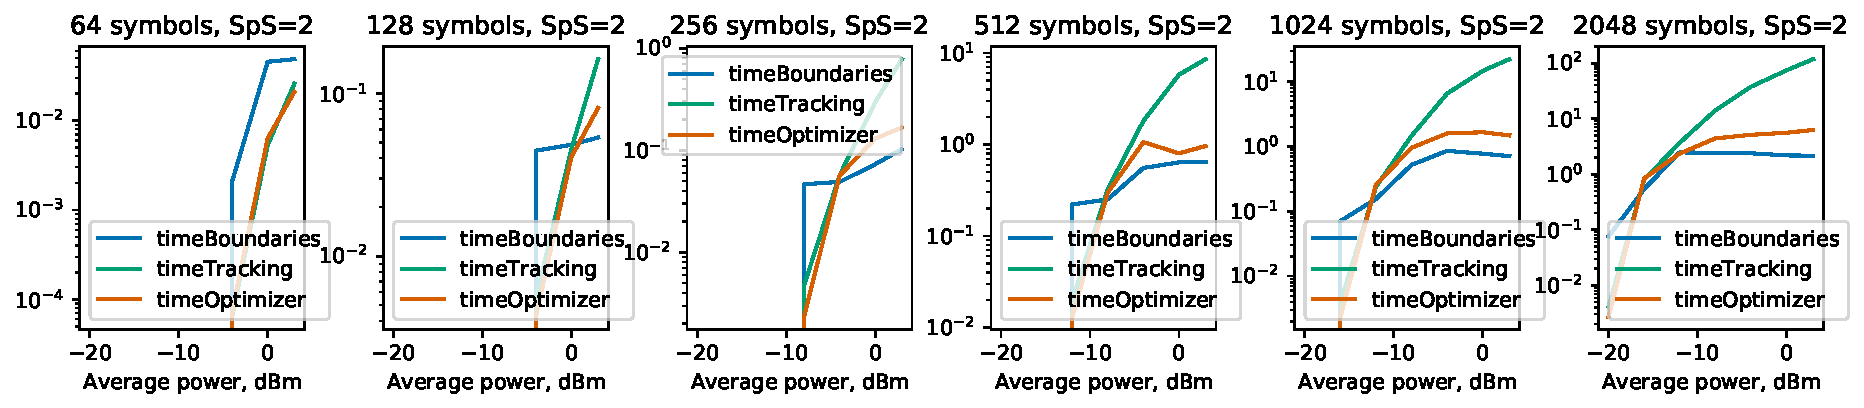
\includegraphics[width=1\linewidth]{images/complexity/PJT_times_132.pdf}
% 	\caption{PJT: operation times (in seconds) for different steps of discrete spectrum search.}
% 	\label{fig:PJTTelecom4}
% \end{figure}